%Authors guidlines: http://royalsocietypublishing.org/instructions-authors
% 2500 words max (includes the title page, abstract, references, acknowledgements and figure/table legends)
% current version is around 3700. I think a big cut down can be done on the references.
% We allow a maximum of 4 displays, only 2 of which can be figures.

\documentclass[12pt,letterpaper]{article}


%Packages
\usepackage{pdflscape}
\usepackage{fixltx2e}
\usepackage{textcomp}
\usepackage{fullpage}
\usepackage{float}
\usepackage{latexsym}
\usepackage{url}
\usepackage{epsfig}
\usepackage{graphicx}
\usepackage{amssymb}
\usepackage{amsmath}
\usepackage{bm}
\usepackage{array}
%\usepackage{mhchem}
\usepackage{ifthen}
\usepackage{caption}
\usepackage{hyperref}
\usepackage{amsthm}
\usepackage{amstext}
\usepackage{enumerate}
\usepackage[osf]{mathpazo}
\usepackage{dcolumn}
\usepackage{lineno}
\usepackage{longtable}

\pagenumbering{arabic}

\newcolumntype{L}[1]{>{\raggedright\let\newline\\\arraybackslash\hspace{0pt}}m{#1}}
\newcolumntype{C}[1]{>{\centering\let\newline\\\arraybackslash\hspace{0pt}}m{#1}}
\newcolumntype{R}[1]{>{\raggedleft\let\newline\\\arraybackslash\hspace{0pt}}m{#1}}

%Pagination style and stuff % NC: Note that these are all syst biol specific.
\linespread{2}
\raggedright
\setlength{\parindent}{0.5in}
\setcounter{secnumdepth}{0} 
\renewcommand{\section}[1]{%
\bigskip
\begin{center}
\begin{Large}
\normalfont\scshape #1
\medskip
\end{Large}
\end{center}}
\renewcommand{\subsection}[1]{%
\bigskip
\begin{center}
\begin{large}
\normalfont\itshape #1
\end{large}
\end{center}}
\renewcommand{\subsubsection}[1]{%
\vspace{2ex}
\noindent
\textit{#1.}---}
\renewcommand{\tableofcontents}{}
%\bibpunct{(}{)}{;}{a}{}{,}

%---------------------------------------------
%
%       START
%
%---------------------------------------------

\begin{document}

%Running head
\begin{flushright}
Version dated: \today
\end{flushright}

\bigskip
\medskip
\begin{center}

\noindent{\Large \bf Do Natural History Documentaries Prompt Public Engagement?} 

\bigskip

\noindent {\normalsize \sc Adam Kane$^1$ and Dario Fernandez-Bellon$^1$}\\
\noindent {\small \it 
$^1$Biological, Earth and Environmental Sciences, University College Cork, Cork, Ireland}\\

\end{center}
\medskip
\noindent{*\bf Corresponding author.} \textit{adam.kane@ucc.ie}\\  
\vspace{1in}

%Line numbering
\modulolinenumbers[1]
\linenumbers

%---------------------------------------------
%
%       ABSTRACT
%
%---------------------------------------------
\begin{abstract}
\end{abstract}

\noindent Key words: conservation, documentaries, public engagement\\


%---------------------------------------------
%
%       INTRODUCTION
%
%---------------------------------------------

\newpage 
\section{Introduction}
We live in the Anthropocene age, a critical time for the planet and the species who inhabit it \cite{rands2010biodiversity}. The effect humanity has on the natural world cannot be overstated given our culpability in causing the so-called the Anthropocene mass extinction event, the worst loss of biodiversity since the dinosaurs perished 65 MYA \cite{barnosky2011has}. We also live in digital age, a time of constant technological change, instant rewards and short attention spans \cite{owen2009internet}. And, although there are signs that people are interested in living sustainably, habitat loss and species extinction continues apace \cite{rands2010biodiversity}. Conservation practitioners are thus faced with the task of alerting the public to the plight of the planet and its many endangered species in a way that is as palatable as it is arresting. 

Nature documentaries have recently shown their potential to fill this role, with viewing figures at record levels \cite{wunder2013taxing,janpol2016does}. These numbers show there is certainly an appeitite among the public for nature. But we wonder whether this medium, in one of its most popular guises, gets the message of conservation across, or if it is lost along the way. And if so, where does that loss occur, so that we may rectify it.

Documentaries readily encounter the dilemma of education versus entertainment which blurs into edutainment \cite{bagust2008screen}. A show that becomes too preachy didactic, or repetitive in its message is sure to lose its audience and, as a consequence, the message it's trying to convey \cite{janpol2016does}. Sir David Attenborough, perhaps the most venerable figure in the history of nature documentary broadcasting, is well aware of this difficulty. In an interview he gave in the 1980s \cite{burgess1984exploring} around the time of The Living Planet he argued, "As a conservationist, I think I would be doing the cause a great disservice if I tacked on to the end of every single programme that I did, a little homily to explain yet again that mankind is wrecking the environment that I have been showing." Rather, his approach has been to showcase the beauty and wonder of the natural world so that the audience will come to appreciate the intrinsic merit of nature and then take some responsibility for its preservation. Any explicit mentions of conservation issues tend to be restricted to a single episode of a documentary run instead of being interspersed throughout \cite{richards2013greening}. This has been a feature of most of his output with the BBC Natural History Unit over the past 40 years. In terms of viewership, his philosophy has been unarguably successful; the latest major broadcast, Planet Earth 2, commanded an audience of around 12 million people per episode in the UK, the highest ever audience for a nature documentary. 

But Sir David's approach has been criticised by commentators who argue the picture painted in his shows is a totally, unrealistic view of a pristine natural world, such that it is disingenuous to talk about the marvels of a critically endangered species without a mention of its perilous state \cite{jeffries2003bbc}. This was best captured by the Guardian journalist George Monbiot, who said, "There are two planet earths. One of them is the complex, morally challenging world in which we live, threatened by ecological collapse. The other is the one we see on the wildlife programmes." Indeed, many of the species featured in his shows are in danger of extinction and any campaign to reverse their decline is likely to be time sensitive \cite{biggs2013legal,turvey2007first}. 

In this work, we wanted to put Sir David's philosophy to the test by assessing how the public respond to his shows in terms of further engagement with nature and matters of conservation. Specifically, we looked to internet-based methods in the form of data from Twitter and Wikipedia to gauge public engagement during the broadcast run of Planet Earth 2 \cite{soriano2017internet}. These methods have proven their worth with respect to the public uptake of species-specific conservation campaigns in the UK \cite{soriano2017internet}. Twitter was chosen to get an understanding of people's instant reactions to the show whereas we used Wikipedia to determine whether people were interested in learning more about the featured species. 




% 2016 Does viewing documentary films affect environmental perceptions and behaviors?
% It has been shown that knowledge does not lead to behavior change in the environmental dimension
% Inconvenient Truth had an effect, but one that was temporary. 
% Documentaries can effect charitable donations 

%---------------------------------------------
%
%       METHODS
%
%---------------------------------------------
\section{Materials and Methods}
We first searched the scripts from the six episodes of Planet Earth 2 for sentences that could be construed as having a conservation theme. This was done indepedently to ensure intercoder reliability. The few discrepanices that resulted were discussed so that we could set out a final set of sentences (See supplementary for script sections). We did this to determine if the script of Planet Earth 2 adhered to Sir David's philosophy described earlier. We then compiled a list of all of the species that were mentioned in the script and assigned each their status on the IUCN Red List. 

We then searched Twitter during the hour each episode was aired and the hour afterwards. We sampled XXX tweets per episode and counted the number mentions of the species that were featured. 

Next, we used the R package \textit{pageviews} to find the daily number of hits the Wikipedia article for each species featured on Planet Earth 2 received over the course of 2016. We searched for the name of the species as it was stated in the script. Our prediction was that the articles for the species featured on the show would see a spike around the air dates relative to the rest of the year. We were able to distinguish the page hits according to whether they came from mobile phone or a desktop search. This enabled us to make the prediciton that more anomalies would be seen from mobile data due to the ubiquity of smart phones and increase in 'dual screening' - watching television whilst using your phone \cite{holz2015m}. 

We used the R package \textit{AnomalyDetection} to pick out anomalies in the detrended time series data we collated from Wikipedia article hits. We looked at two different senstivities, at 1\% and 2\%. A 1\% sensitivity meant there could be a maximum of 3 anomalous days of hits for an article because it is based on a sample of 365 days, at 2\% there are a maximum of 7 possible days. Of course, there can be fewer extremes or even none. We counted the number of times an article's anomalous day occurred either during the day of broadcast or the day after broadcast of an episode of Planet Earth 2 at both sensitivty levels. We recorded mobile access to the site, desktop access and a combination of the two. We also ran the same analysis using the USA airdates for the show but over a shorter time scale, from January to April 2017.   

%First we looked at the potential of documentaries to impact / generate public awareness a.Sequence time (or no words) and number of original tweets and wiki hits. Then we look at whether docs are actually reflecting what occurs in the natural world, or as recent criticism suggests, represents a fictitious picture of the state of the plane. a. IUCN vertebrate status -> reflected in script? -> reflected in twitter volume or sentiment?-> reflected in wiki hits? b.Total time / words dedicated to cons messages (including overview sequences) c.Figure with map of distribution of stories, taxa breakdown and IUCN status breakdown. Finally, we look at whether this awareness actually results in engagement and has an impact on conservation issues. Case studies of specific sequences and web hits/donations to relevant charities.




%wiki ~ conservation message (binary) + taxa level (categorical) + sequence time + diaries presence (binary)? + relative popularity from wiki + no. of mentions + twitter sentiment?

%Combine data from sequence time with time during diaries

%Measure each species' article during 2015 and use as a baseline of popularity to see the effect of the series in 2016.

%If he doesn't mention the species name it means people don't search for the species by name, rather more generically, and on Wikipedia this means they won't see the figure with IUCN status. 

%---------------------------------------------
%
%       RESULTS
%
%---------------------------------------------


\section{Results}
In total we analysed 93 distinct animals that featured in the script of Planet Earth 2 over the six episodes. In addition, five species featured in two separate episodes, indri, giant otter, lion, termite and peregrine falcon, giving a total of 98 animal species. As expected there were few explicit discussions of conservation across the series. Notably, the IUCN status of the featured animals was never mentioned.  
\begin{figure}[H]
\centering
    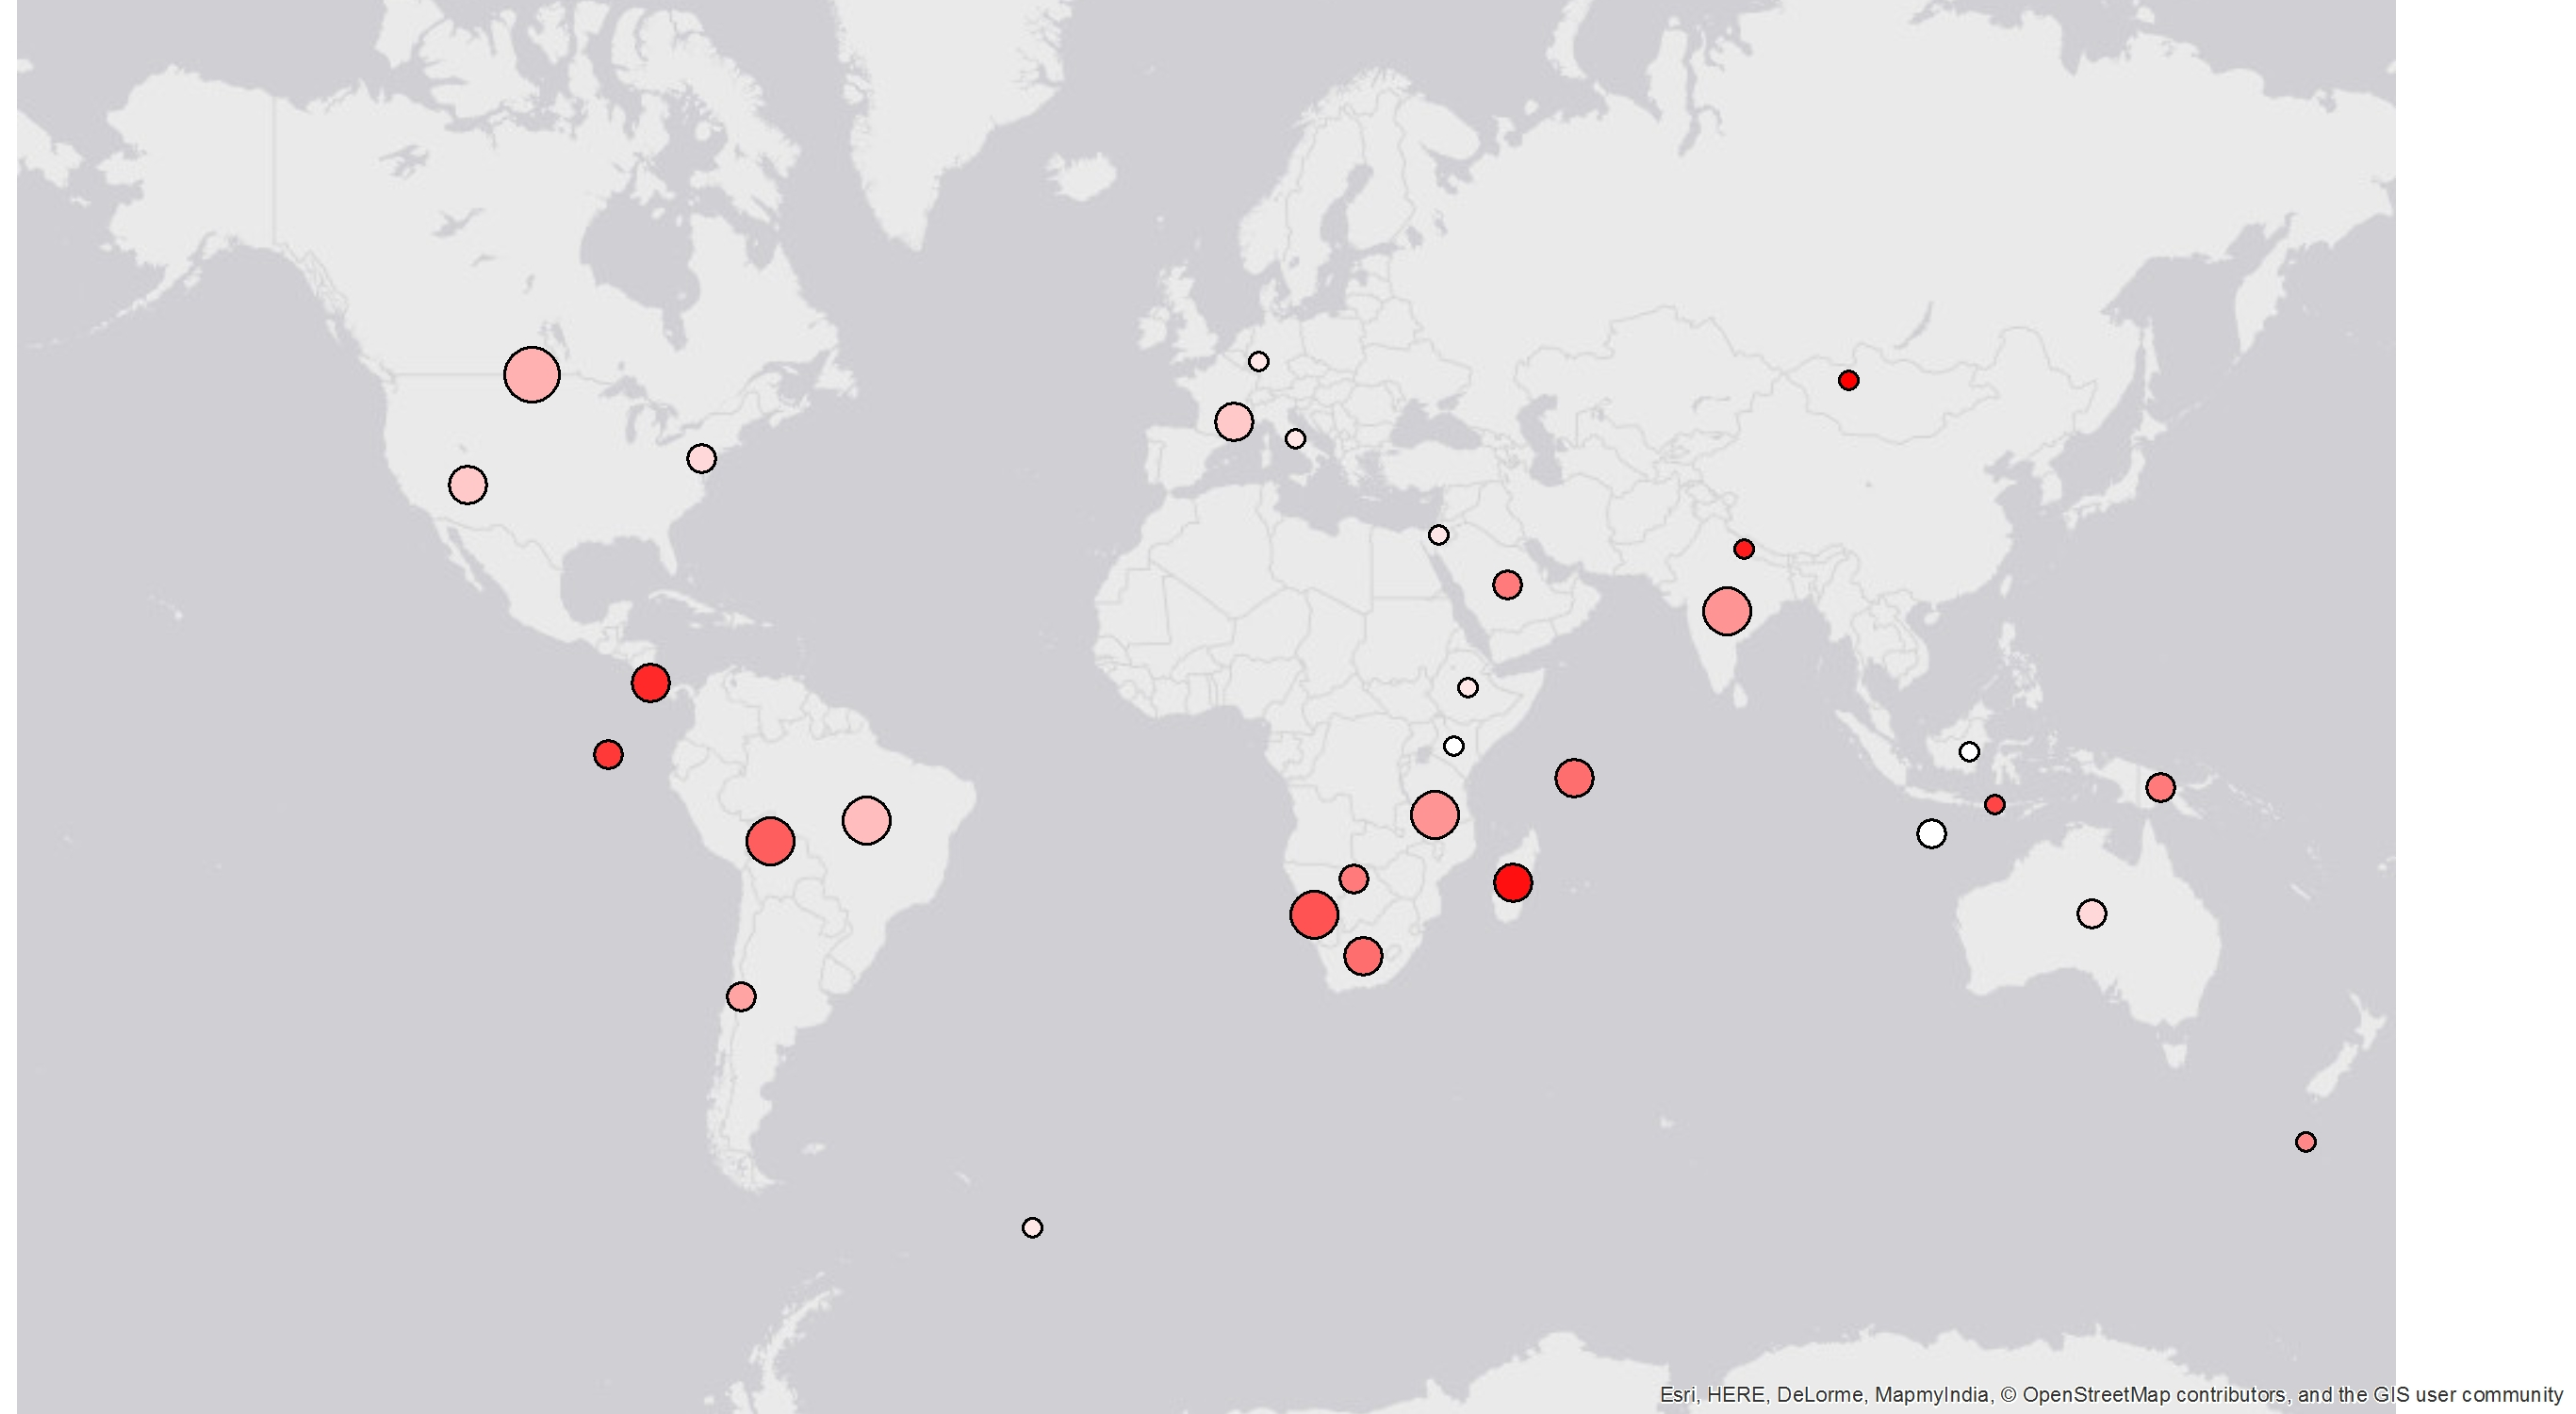
\includegraphics[keepaspectratio, totalheight=0.5 \textheight]{map2.jpg}
\caption{Average IUCN status of species featured on Planet Earth 2}
\label{info.diff}
\end{figure}

\begin{table}
    \begin{tabular}{cccc} 
   \hline
    Country & Sensitivity & Access   & Percentage of anomalies \\ \hline
    UK      & 1\%         & Mobile   & 54                      \\
    UK      & 1\%         & Desktop  & 34                      \\
    UK      & 1\%         & Combined & 45                      \\
    UK      & 2\%         & Mobile   & 65                      \\
    UK      & 2\%         & Desktop  & 44                      \\
    UK      & 2\%         & Combined & 57                      \\ \hline
    USA     & 1\%         & Mobile   & 27                      \\ 
    USA     & 1\%         & Desktop  & 10                      \\
    USA     & 1\%         & Combined & 22                      \\
    USA     & 2\%         & Mobile   & 37                      \\
    USA     & 2\%         & Desktop  & 17                      \\
    USA     & 2\%         & Combined & 30                      \\ \hline
    \end{tabular}
\end{table}
%\begin{table}[]
%\centering
%\caption{Species featured on Planet Earth 2 with associated search terms and IUCN status}
%\label{my-label}
%\begin{tabular}{ll} \hline
%\begin{center}
%\begin{longtable}{ll}
%\caption[Species featured on Planet Earth 2 with associated search terms and IUCN status]
%{Species featured on Planet Earth 2 with associated search terms and IUCN status} \label{Species} \\

%\hline \multicolumn{1}{c}{\textbf{Search Terms}} & \multicolumn{1}{c}{\textbf{IUCN Status}} \\ \hline 
%\endfirsthead


%\multicolumn{2}{c}%
%{{\bfseries \tablename\ \thetable{} -- continued from previous page}} \\
%\hline \multicolumn{1}{c}{\textbf{Search terms}} &
%\multicolumn{1}{c}{\textbf{IUCN Status}}  \\ \hline 
%\endhead

%\hline \multicolumn{2}{r}{{Continued on next page}} \\ \hline
%\endfoot

%\hline \hline
%\endlastfoot

%Sloth, Pygmy three toed sloth                   & CR          \\
%Komodo dragon                                   & VU          \\
%Lemur                                           &  -           \\
%Sifaka, Verraux's Sifaka                        & EN          \\
%Iguana, Marine Iguana                           & VU          \\
%Snake, Galapagos racer                          & NA          \\
%Seabird                                         & -           \\
%Albatross, Buller's albatross                   & NT          \\
%Tern, Fairy tern                                & VU          \\
%Fody, Seychelles fody                           & NT          \\
%Noddy (tern)                                    & LC          \\
%Crab, Christmas Island red crab                 & NA          \\
%Ant, Yellow crazy ant                           & NA          \\
%Penguin, Chinstrap penguin                      & LC          \\
%Ibex, Nubian ibex                               & VU          \\
%Fox, Red fox                                    & LC          \\
%Eagle, Golden eagle                             & LC          \\
%Bear, Grizzly bear                              & LC          \\
%Bobcat                                          & LC          \\
%Groundsel, Cabbage groundsel                    & LC          \\
%Viscacha, Mountain viscacha                     & LC          \\
%Flamingo, Chilean Flamingo                      & NT          \\
%Leopard, Snow leopard                           & VU,EN       \\
%Monkey, Spider Monkey, Geoffroy's spider monkey & EN          \\
%Lizard, Draco lizard                            & NA          \\
%Hummingbird, Sword-billed hummingbird           & LC          \\
%Dolphin, River dolphin                          & DD          \\
%Jaguar                                          & NT          \\
%Frog, Glass frog, Fleischmann's Glass frog      & LC          \\
%Beetle, Click beetle                            & NA          \\
%Worm, Railroad worm                             & NA          \\
%Bird-of-paradise, Red bird-of-paradise          & NT          \\
%Wilson's bird-of-paradise                       & NT          \\
%Indri                                           & CR          \\
%Lion                                            & VU          \\
%Oryx, East African oryx                         & NT          \\
%Giraffe                                         & VU          \\
%Hawk, Harris's hawk                             & LC          \\
%Squirrel, Ground squirrel                       & ID?         \\
%Butcherbird, Shrike, Loggerhead shrike          & LC          \\
%Locust                                          & ID?         \\
%Zebra                                           & NT          \\
%Elephant, African elephant                      & VU          \\
%Sandgrouse                                      & LC          \\
%Mustang                                         & NA          \\
%Lizard, Shovel snouted lizard                   & NA          \\
%Mole, Golden mole                               & ID?         \\
%Bat, Desert long-eared bat                      & LC          \\
%Beetle, Darkling beetle                         & NA          \\
%Antelope, Saiga antelope                        & CR          \\
%Buffalo, African buffalo                        & LC          \\
%Mouse, Harvest mouse, Micromys                  & LC          \\
%Owl, Barn owl                                   & LC          \\
%Bee-eater, Southern carmine bee-eater           & LC          \\
%Bustard, Kori bustard                           & NT          \\
%Ostrich                                         & LC          \\
%Serval                                          & LC          \\
%Rat, Southern African vlei rat                  & LC          \\
%Wildebeest, Blue Wildebeest                     & LC          \\
%Widow bird, Jackson's widowbird                 & NT          \\
%Grasscutter ant                                 & ID?         \\
%Termite, Compass termites                       & ID?         \\
%Anteater, Giant anteater                        & VU          \\
%Bison                                           & NT          \\
%Caribou                                         & VU          \\
%Wolf, Grey wolf                                 & LC          \\
%Langur, Gray Langur                             & LC          \\
%Falcon, Peregrine Falcon                        & LC          \\
%Pigeon                                          & LC          \\
%Starling, Common starling                       & LC          \\
%Bowerbird, Great bowerbird                      & LC          \\
%Racoon                                          & LC          \\
%Macaque, Rhesus macaque                         & LC          \\
%Hyena, Spotted hyena                            & LC          \\
%Catfish, Wels catfish                           & LC          \\
%Turtle, Hawksbill turtle                        & CR          \\
%Otter, Smooth-coated otter                      & VU         
%\end{tabular}
%\end{table}
%\end{longtable}
%\end{center}


%---------------------------------------------
%
%       DISCUSSION
%
%---------------------------------------------

\section{Discussion}

%Biology letters various stuff
\section{Ethics statement}
N/A
\section{Data accessibility statement}
All data and analysis code is available on GitHub (\url{https://github.com/kanead}).
\section{Authors' Contributions}
All authors approved the final version of the manuscript.
\section{Competing Interests}
We have no competing interests.
\section{Acknowledgments}
We thank Sir David and Amy Cooke for support.

\bibliographystyle{vancouver}
\bibliography{References}

%END
\end{document}


%"As a conservationist, I think I would be doing the cause a great disservice if I tacked on to the end of every single programme that I did, a little homily to explain yet again that mankind is wrecking the environment that I have been showing. My job as a natural history film make is to convey the reality of the environment so that people will recognise its value, its interest, its intrinsic merit and feel some responsibility for it. After that has been done, then the various pressure groups can get at them through their own channels and ask them to send a donation to, let us say, the World Wildlife Fund." \cite{burgess1984exploring}.

% George Monbiot

%"The loss of wilderness is a truth so sad, so overwhelming that, to reflect reality, it would need to be the subject of every wildlife film. That, of course, would be neither entertaining nor ultimately dramatic. So it seems that as filmmakers we are doomed either to fail our audience or fail our cause."
%Stephen Mills (1997)